\chapter{Results}
\label{chap:results}

\section{Interface}
As mentioned in the previous chapter, SketchMeshVR does not make use of any menus and instead solely relies on different combinations of button presses to differentiate between the multiple available modeling actions. This does require more effort from the user in order to keep track of the selected editing modes, but at the same time keeps the interface cleaner. In order to guide the user when drawing strokes, SketchMeshVR provides visual feedback on the positions that will be used to create a stroke. In case of the drawing and curve deformation modes this means that the user sees the position of the controller and in case of all other modes the user will see the position of the controller plus a ray shooting from it (the ray ends at any intersections it has with the existing model). Figures~\ref{fig:interface}(a) and (b) show what this looks like.

\begin{figure}[!h]
    \centering
    \setlength{\tabcolsep}{0.0130\linewidth}
    \begin{tabular}{@{}cc@{}}
    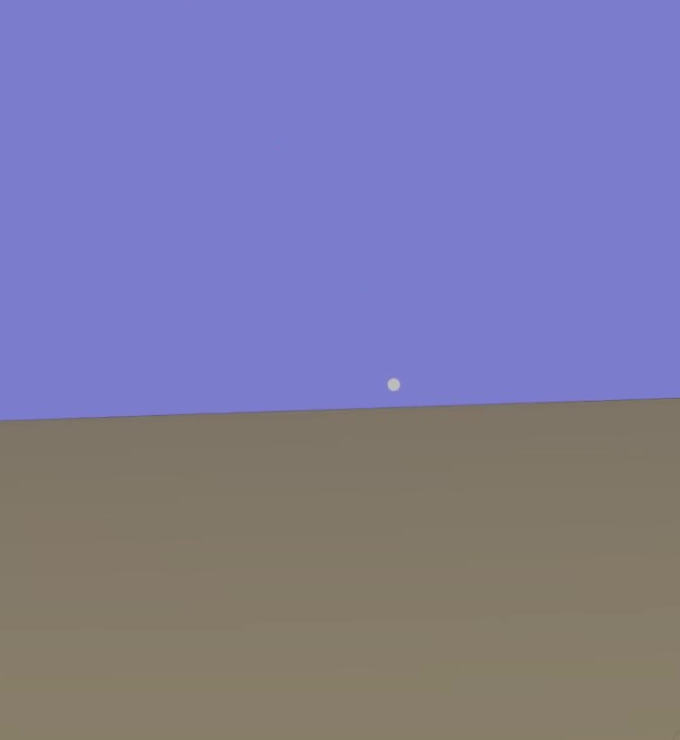
\includegraphics[width=0.3\linewidth]{figures/interface_point}&
  	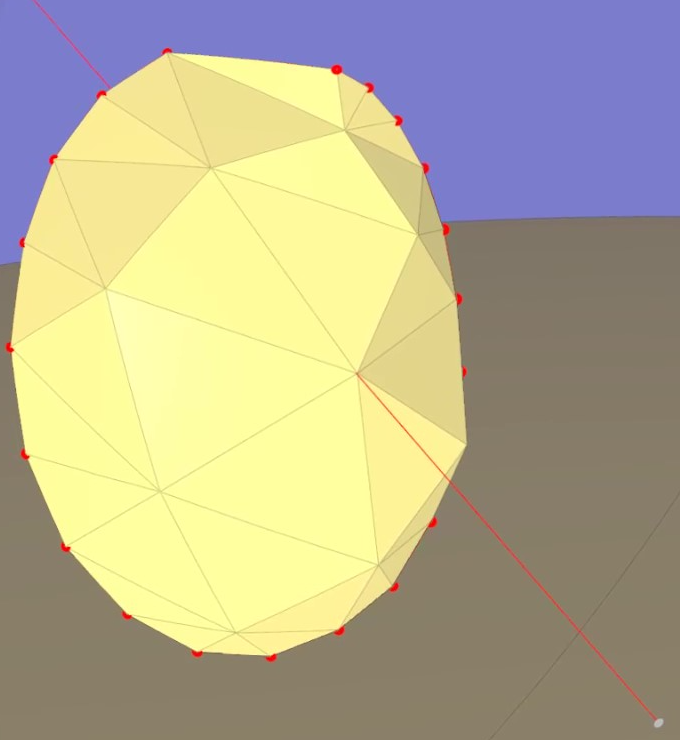
\includegraphics[width=0.3\linewidth]{figures/interface_ray}\\
    (a)&(b)\\
    \end{tabular}
    \caption[SketchMeshVR interface]{SketchMeshVR interface.
    	  \textup{(a)} Controller reference point that is displayed in drawing and deformation mode.
			  \textup{(b)} Controller and ray reference that are displayed in all other editing modes. 
      \label{fig:interface}}
\end{figure}
 
\section{User review}
Our program has been tested by users that had none to little prior experience with 3D modeling and also had none to little experience with VR. The test users were requested to first try and recreate one of the example models from Figures~\ref{fig:recreate_teddy} or~\ref{fig:recreate_dolphin} using SketchMeshVR and then to recreate the same model in the non-VR version of the software. Users reported that although it took some initial effort to get acquainted with the controls, it was very easy to learn how to use SketchMeshVR. They also reported that the immersive nature of VR made the interaction with the created mesh much more impressive compared to the non-VR SketchMesh. 

Although the users had experience with creating the given models when they modeled them in non-VR, it took them longer to recreate the model than when using SketchMeshVR. Especially performing extrusions takes significantly less time in VR than in non-VR, due to the ability to specify silhouette strokes in 3D space. Curve deformation also proved easier and faster to perform in VR, especially when there are multiple control curves close to eachother (the projection method that is used in non-VR can lead to the selection of different curves from what the user expected). Figures~\ref{fig:recreate_teddy} and~\ref{fig:recreate_dolphin} show side-by-side comparisons of the example models that were given to the test users, and the models that they created in both the non-VR and VR versions of our software. As you can see, the users managed to create models that were similar to the example models that were provided to them. The recreated teddy models do not show much difference between the VR and non-VR tool, apart from the time it took to create them. The recreated dolphin model does show a difference in detail between the version creaetd in VR and non-VR, with the non-VR version showing more resemblance with the example model. With SketchMeshVR users had difficulty creating the typical dolphin head shape and the sharp endings of the fins due to the lack of a sharp deformation tool. Users reported that the addition of this tool mode would greatly increase the artistic possibilities of SketchMeshVR.

Figure~\ref{fig:recreate_turtle_bunny} shows two further models that the test users created in SketchMeshVR, alongside the example models that were provided to them. While creating the turtle model, the user reported that the lack of a mesh navigation option was preventing them from adding the hind legs to the turtle since the user could not walk to the backside due to a desk being in the way. Future improvements of SketchMeshVR should definitely include this option in order to avoid this problem and also to simplify mesh editing when the mesh is either close to the physical floor or out of reach for the user.

While creating these models, users did not experience any fatigue in their hands. When using the software for a prolonged period though (15 minutes or more), users started to feel tiredness in their arms due to the relatively large body movement as compared to mouse movement. Users did not experience fatigue from the VR rendering while using the application and reported that they found the rendering to be very smooth. However, after prolonged wear of the headset some users reported an uncomfortable feeling due to the Oculus Rift headset pressing on the face. 


\begin{figure}[!h]
    \centering
    \setlength{\tabcolsep}{0.0130\linewidth}
    \begin{tabular}{@{}ccc@{}}
    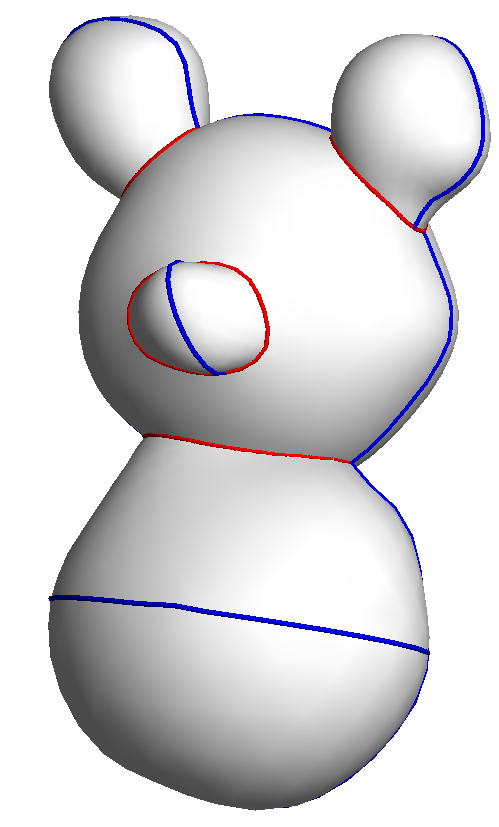
\includegraphics[width=0.3\linewidth]{figures/example_model_figure}&
  	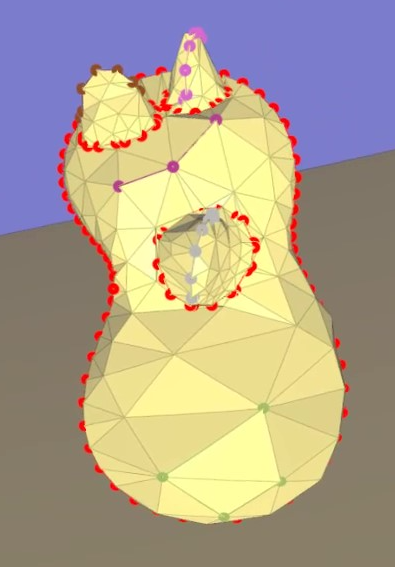
\includegraphics[width=0.3\linewidth]{figures/results_teddy_model1}&
  	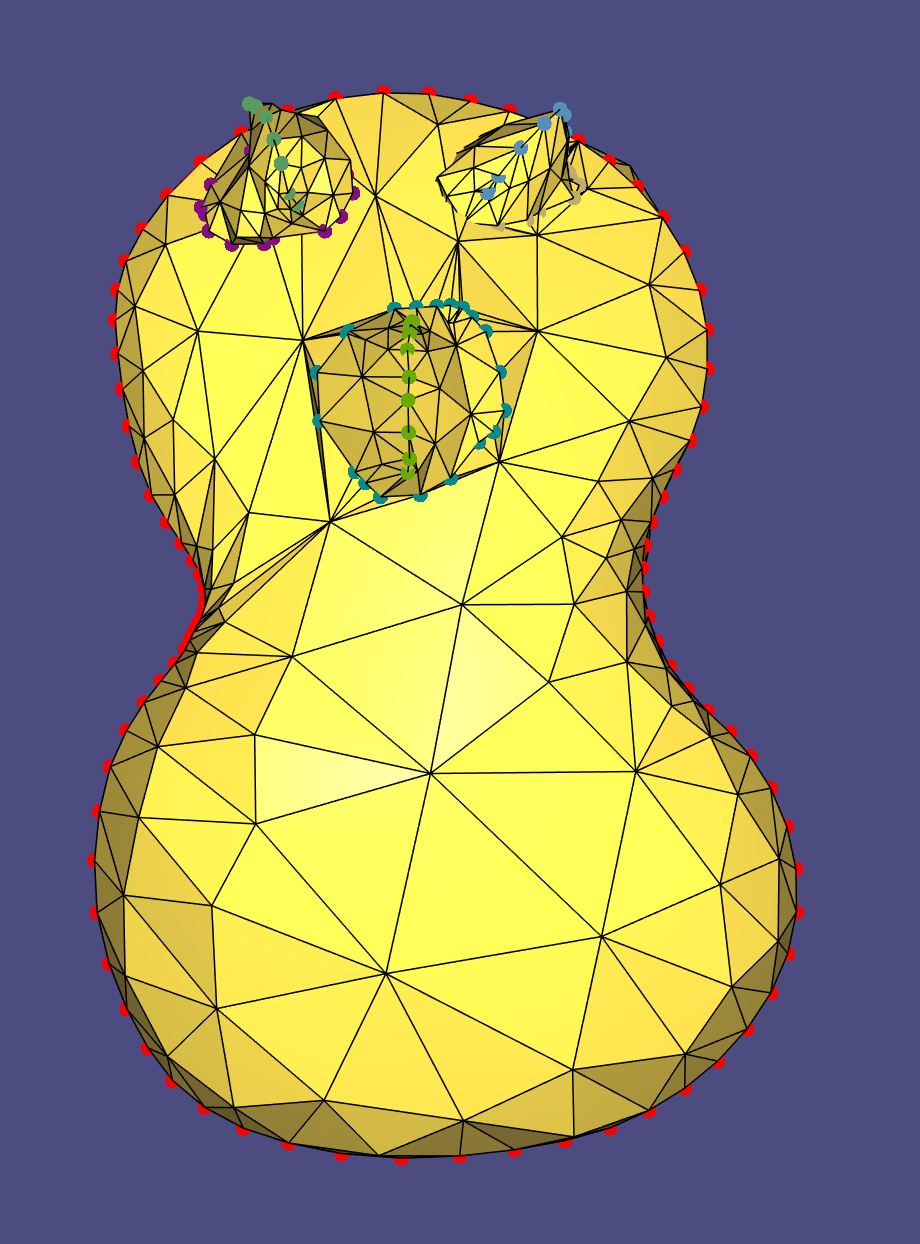
\includegraphics[width=0.3\linewidth]{figures/results_teddy_model_nonVR}\\

    (a)&(b)&(c)\\
    \end{tabular}
    \caption[SketchMeshVR simplified teddy bear model]{SketchMeshVR recreating models.
    	  \textup{(a)} Example mesh of a simplified teddy bear.
	  \textup{(b)} Resulting recreated model made in VR (took 6 minutes to complete).
	  \textup{(c)} Resulting recreated model made in non-VR (took 8 minutes to complete).
      \label{fig:recreate_teddy}}
\end{figure}


\begin{figure}[!h]
    \centering
    \setlength{\tabcolsep}{0.0130\linewidth}
    \begin{tabular}{@{}ccc@{}}
    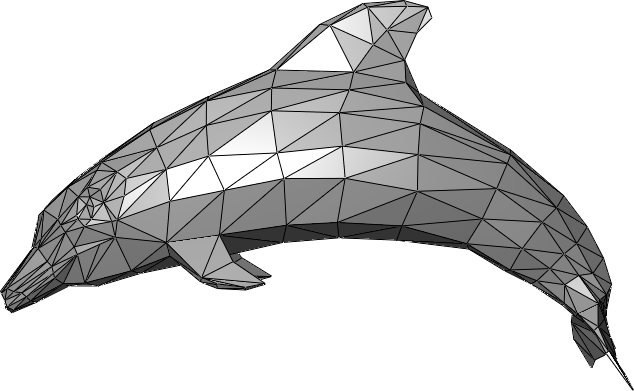
\includegraphics[width=0.3\linewidth]{figures/example_model_dolphin}&
  	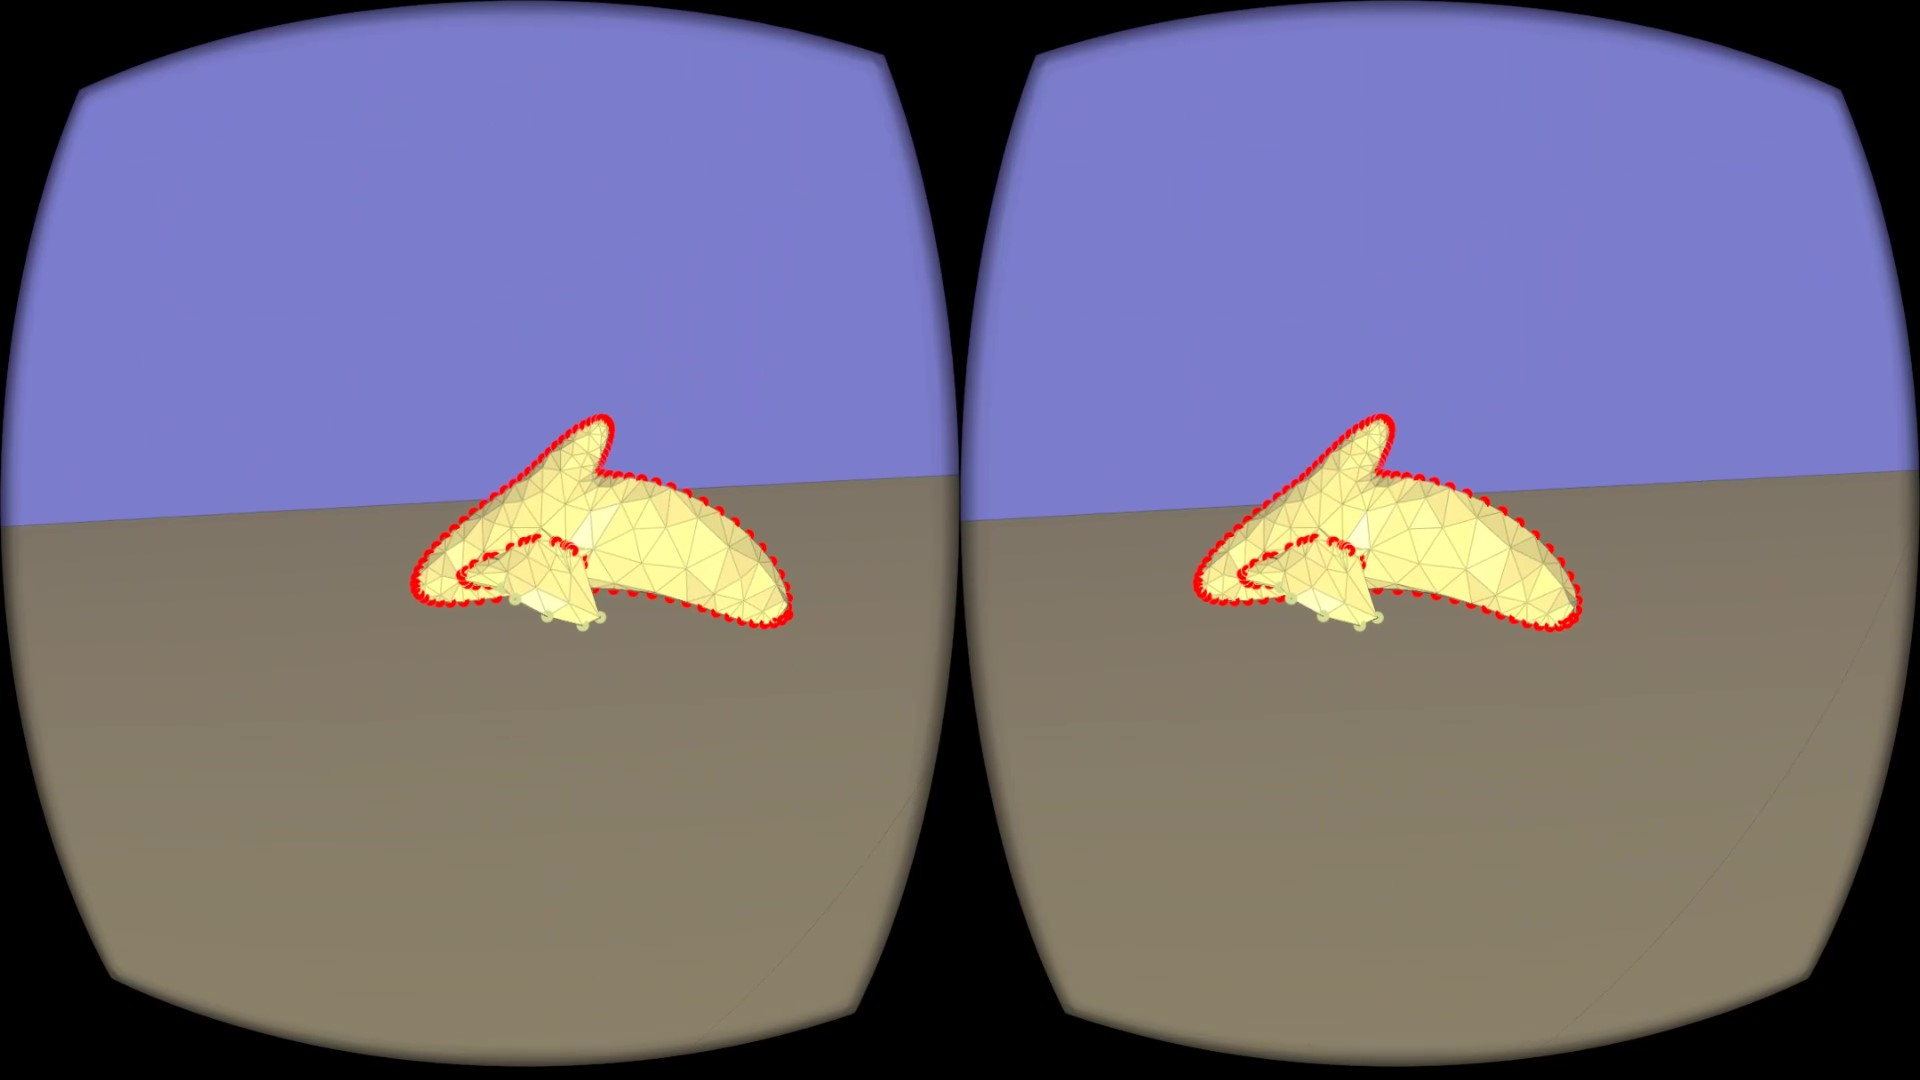
\includegraphics[width=0.3\linewidth]{figures/results_dolphin_model}&
  	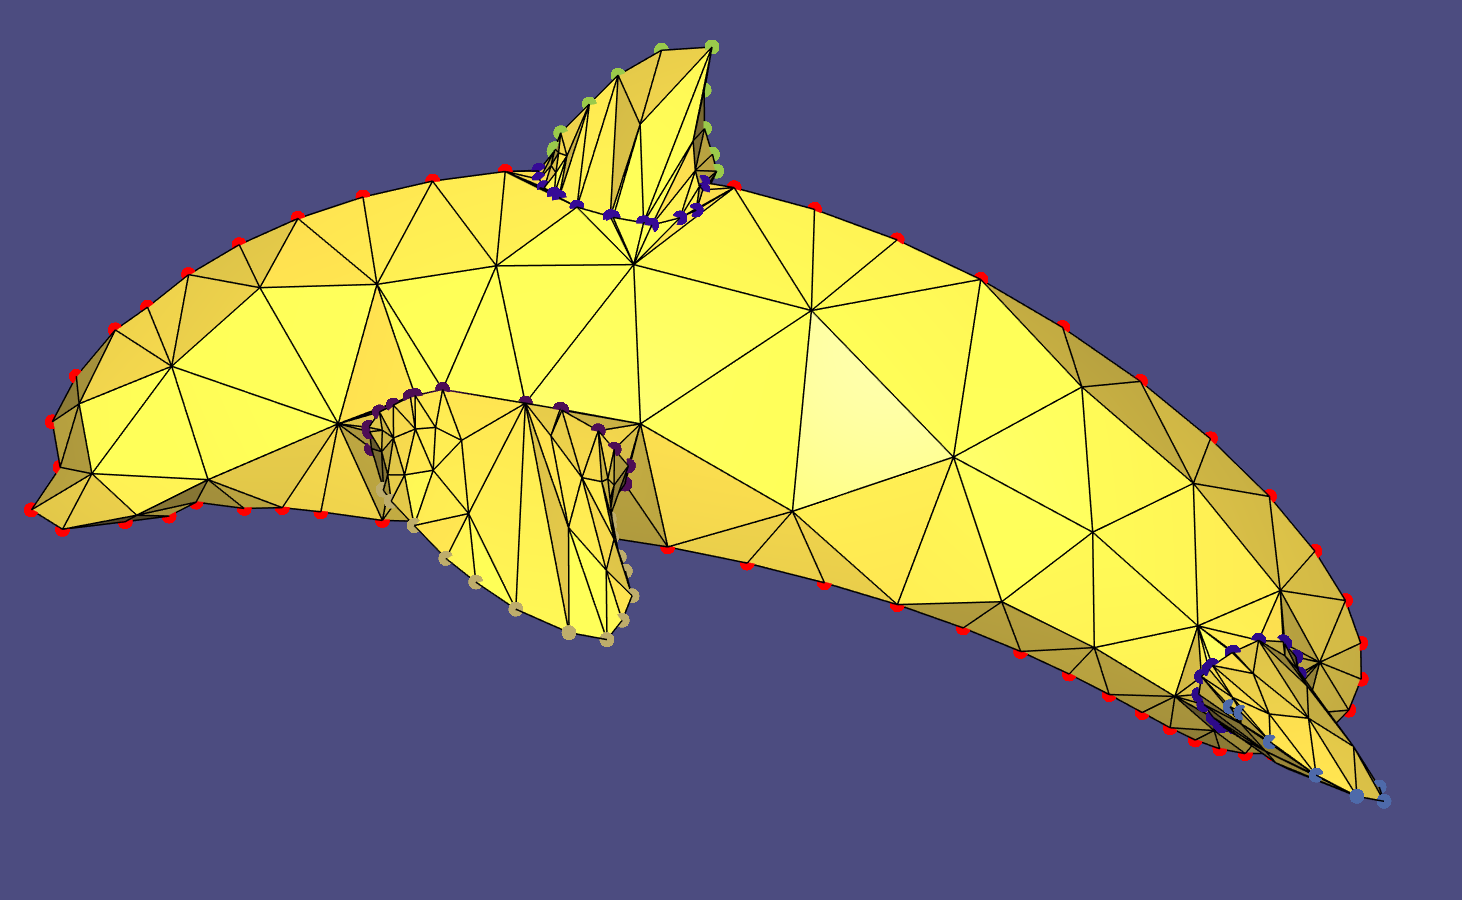
\includegraphics[width=0.3\linewidth]{figures/results_dolphin_model_nonVR}\\

    (a)&(b)&(c)\\
    \end{tabular}
    \caption[SketchMeshVR dolphin model]{SketchMeshVR recreating models.
    	  \textup{(a)} Example simplified mesh of a dolphin.
	  \textup{(b)} Resulting recreated model made in VR (took 7 minutes to complete).
	  \textup{(c)} Resulting recreated model made in non-VR (took 12 minutes to complete).
      \label{fig:recreate_dolphin}}
\end{figure}

\begin{figure}[!h]
    \centering
    \setlength{\tabcolsep}{0.0130\linewidth}
    \begin{tabular}{@{}cccc@{}}
    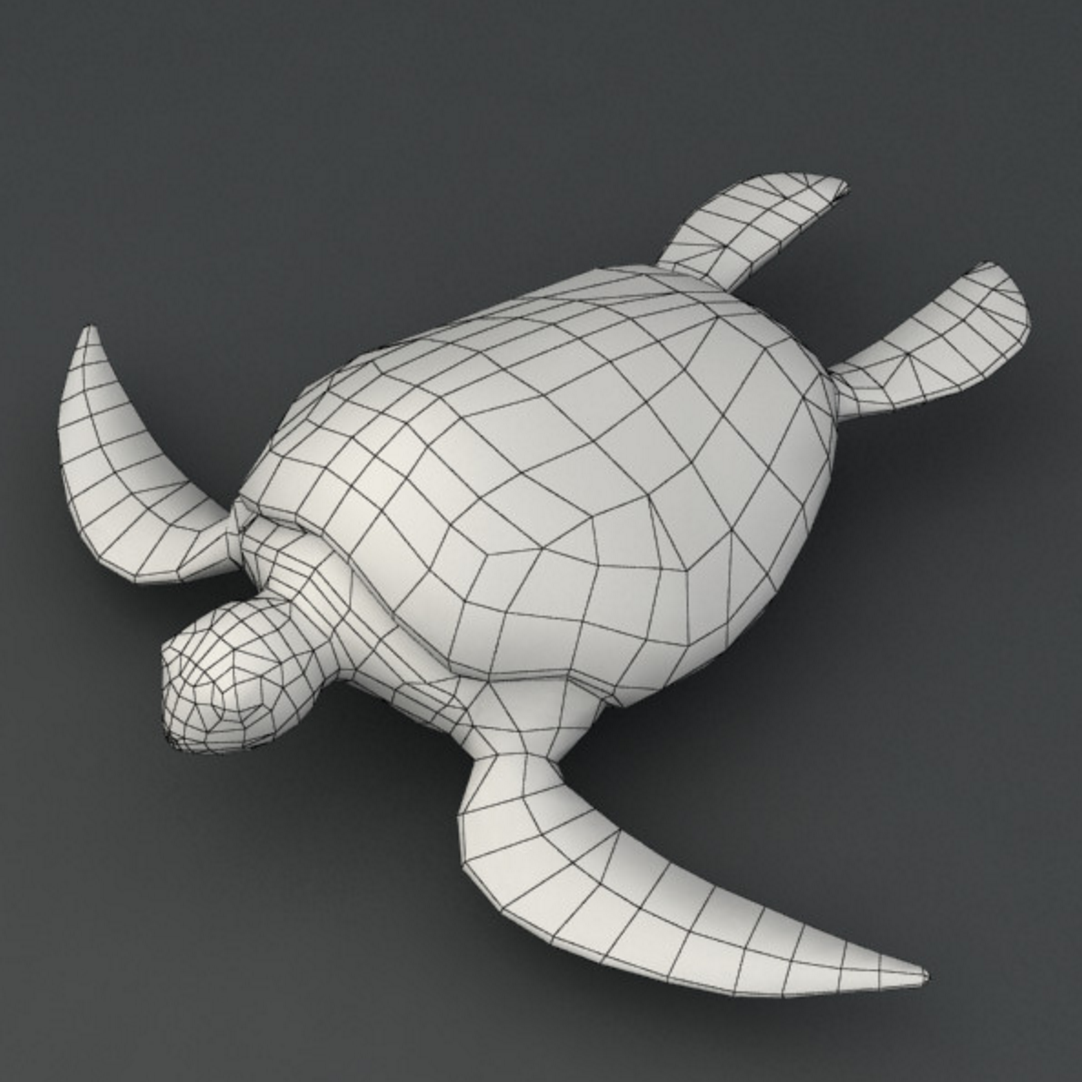
\includegraphics[width=0.45\linewidth]{figures/example_model_turtle}&
        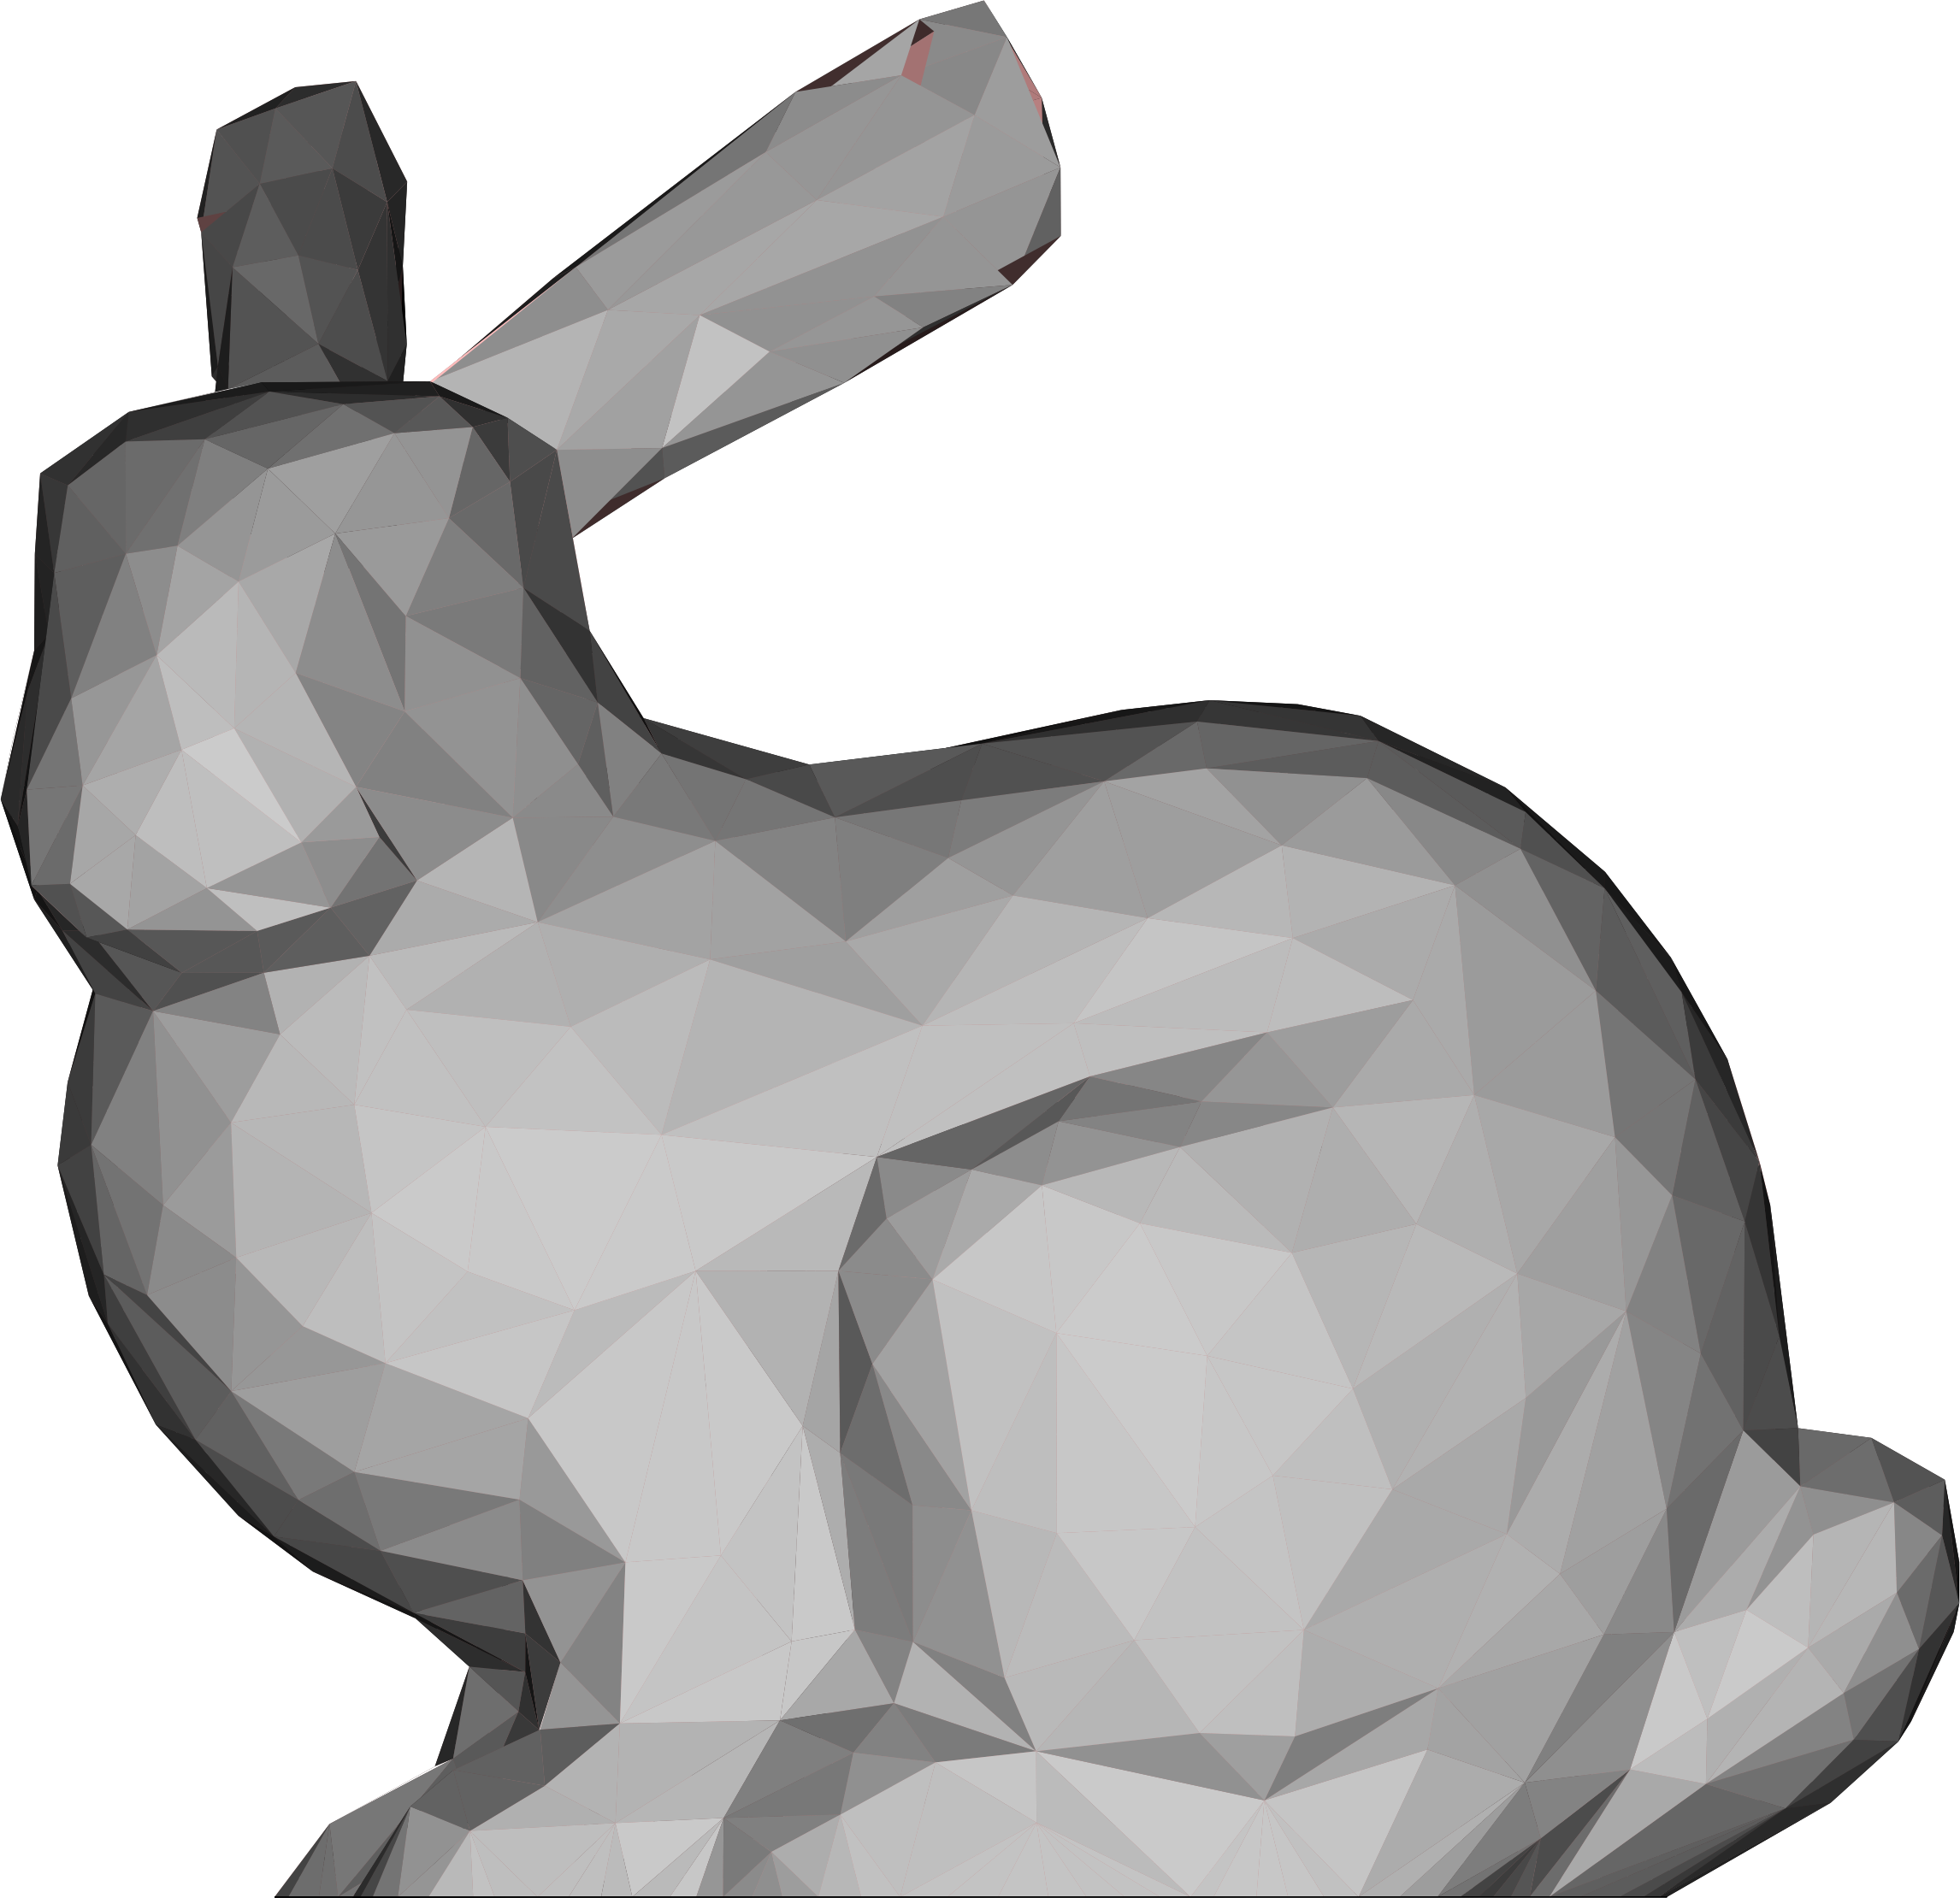
\includegraphics[width=0.45\linewidth]{figures/example_model_bunny}\\
    (a)&(b)\\

  	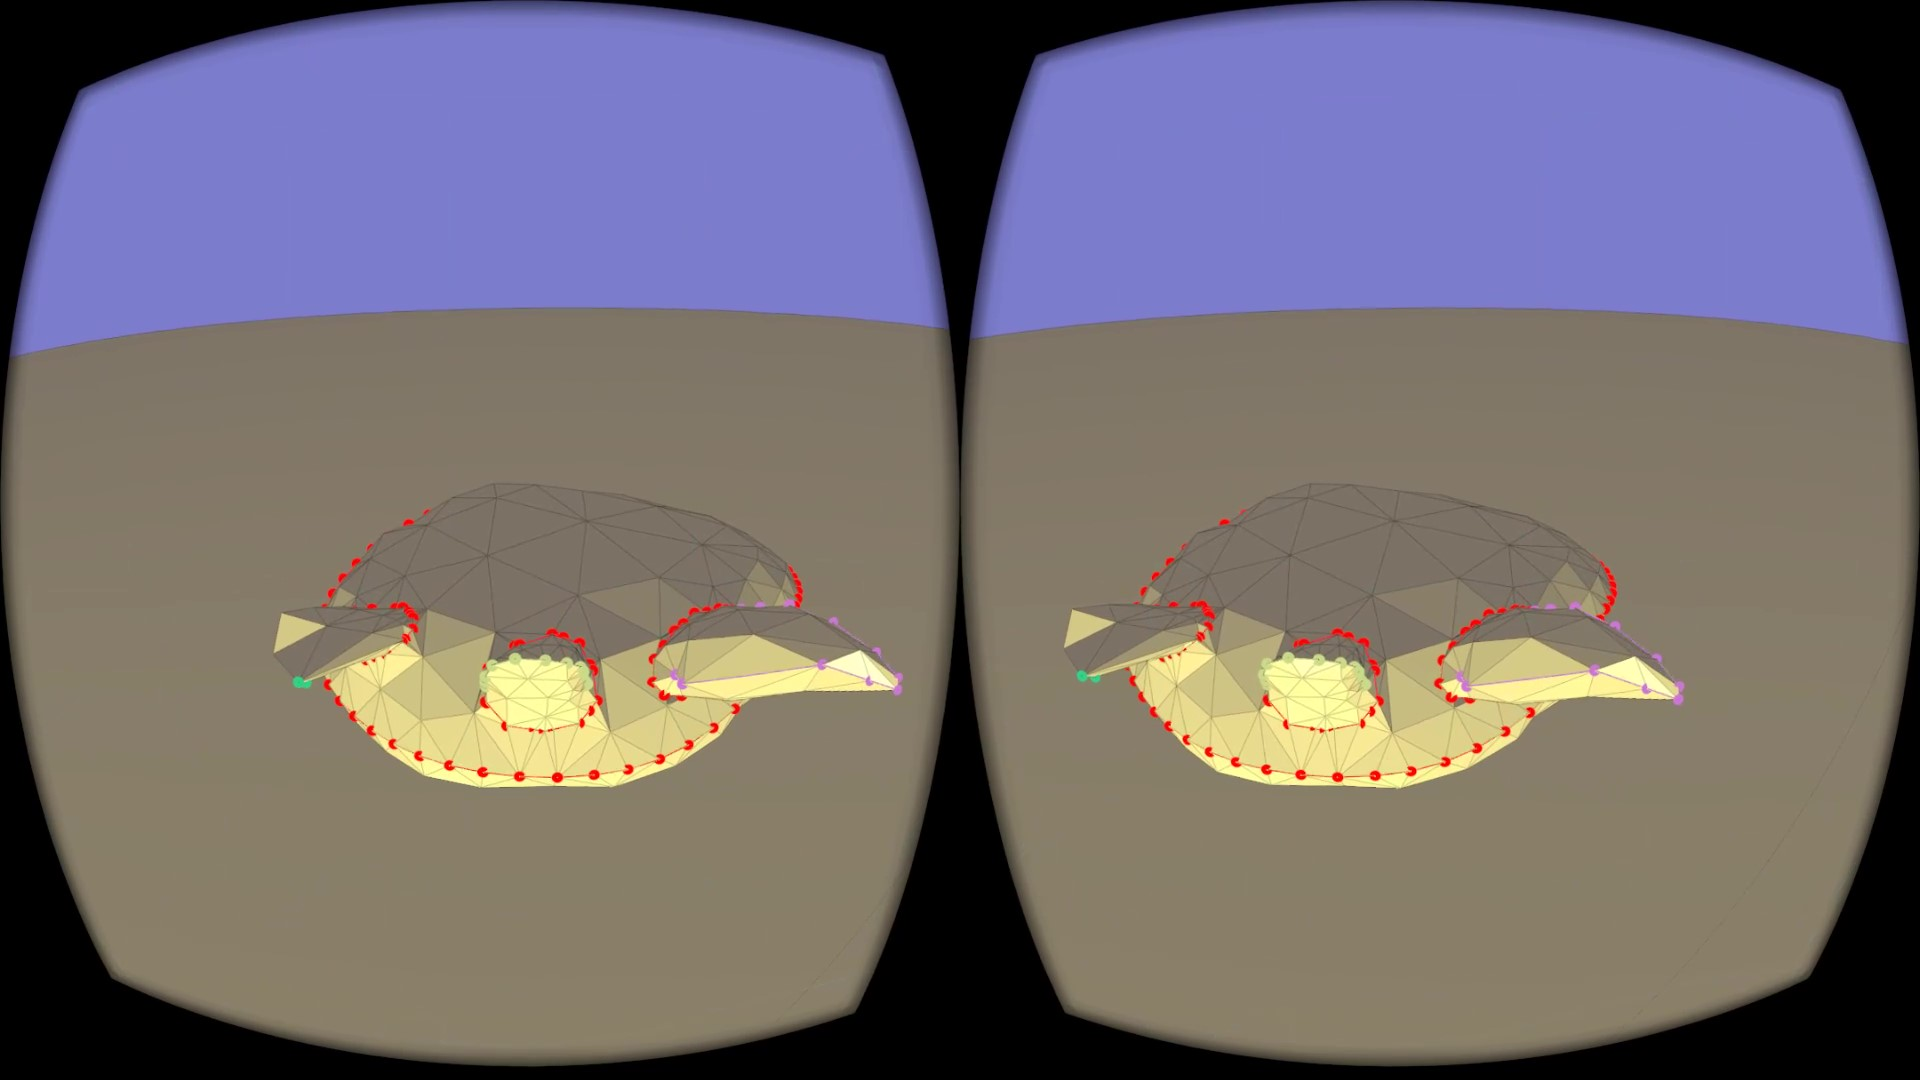
\includegraphics[width=0.48\linewidth]{figures/results_turtle_model}&
  	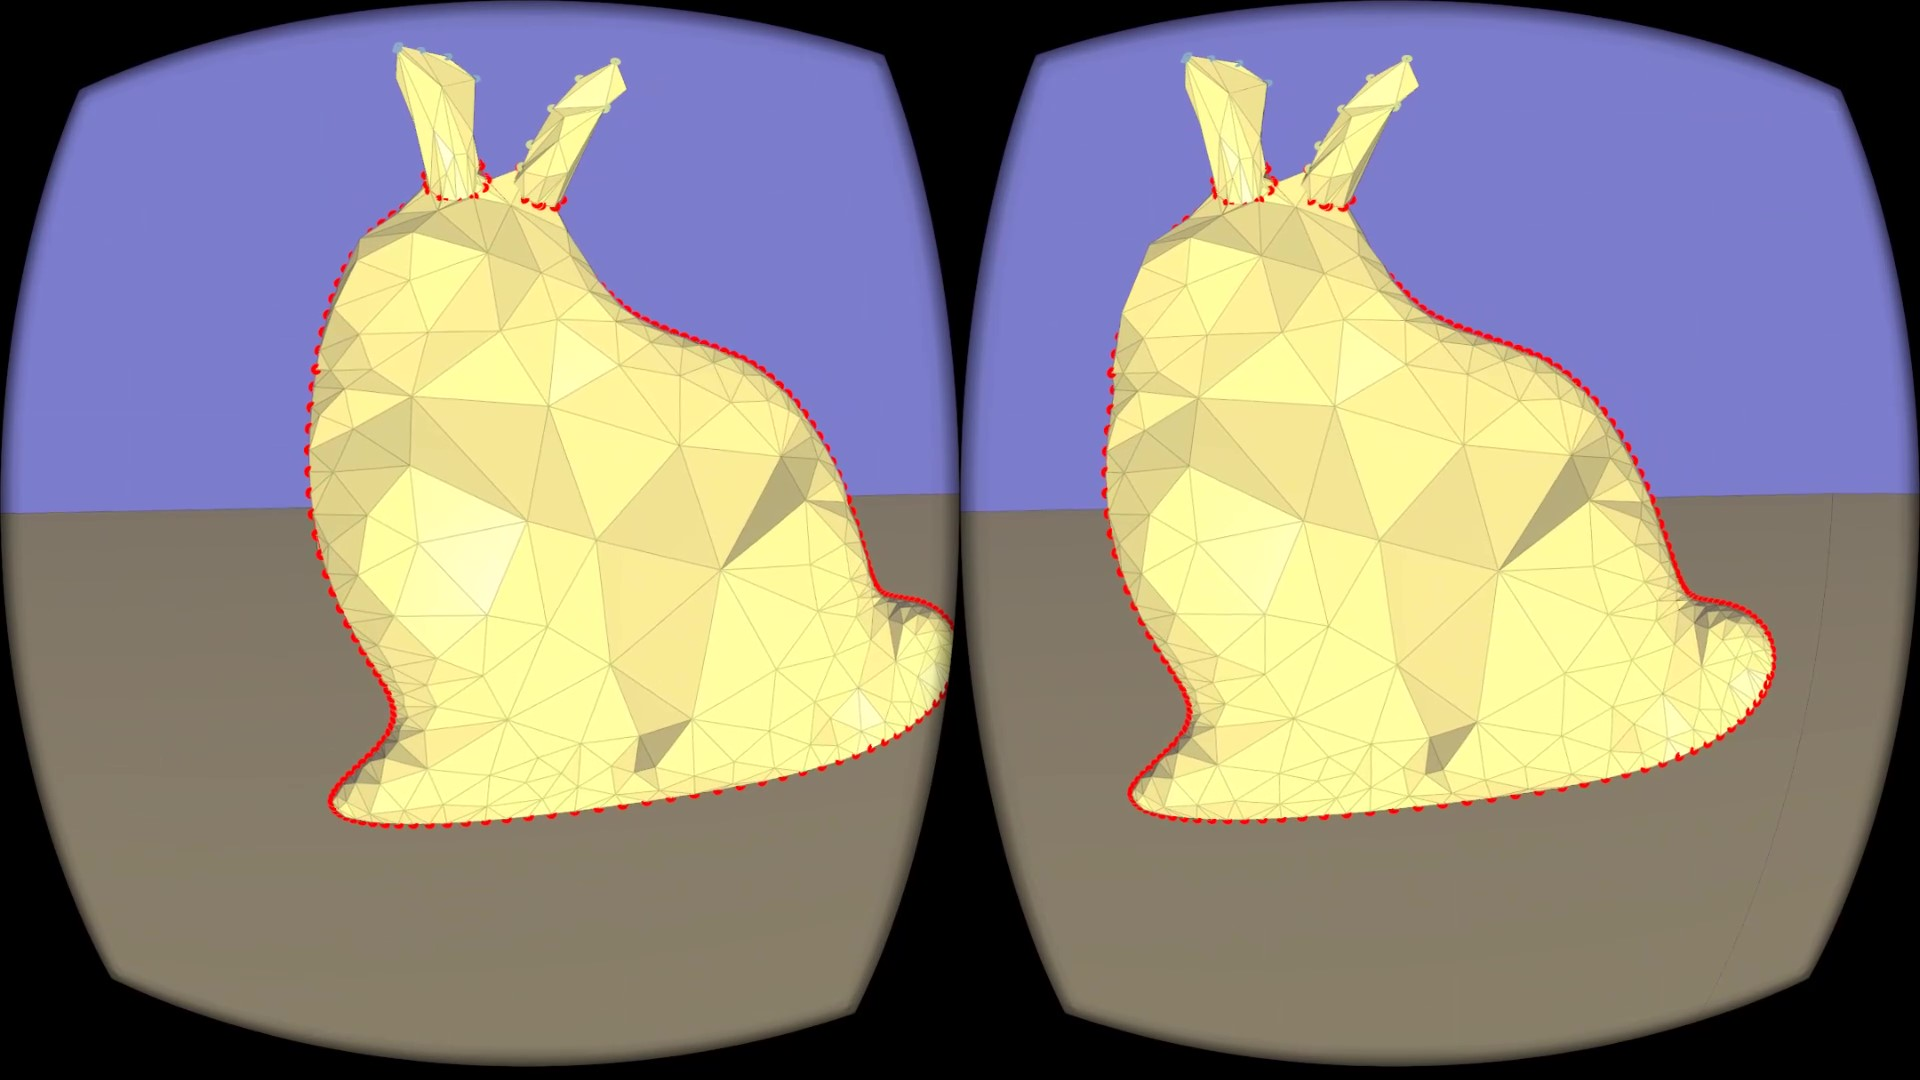
\includegraphics[width=0.48\linewidth]{figures/results_bunny_model}\\
(c)&(d)\\
    \end{tabular}
    \caption[SketchMeshVR turtle and Stanford bunny model]{SketchMeshVR recreating models.
    	  \textup{(a)} Example mesh of a turtle.
    	  \textup{(b)} Example mesh of the Stanford bunny.
	  \textup{(c)} Resulting recreated model made in VR (took 5 minutes to complete).
	  \textup{(d)} Resulting recreated model made in VR (took 9 minutes to complete).
      \label{fig:recreate_turtle_bunny}}
\end{figure}

Also users reported that they found the modeling to be considerably more effortless in VR, as it requires less intermediate navigation of the mesh between modeling steps (for example before drawing the extrusion silhouette or making a diagonal cut there is no need to rotate the mesh in VR). However they did also remark that actions that required larger precision, such as defining additional control curves, were easier to perform with the mouse than in VR.
Additionally users noted that the possibility to define strokes in an additional dimension provides added artistic freedom, for example when defining the extrusion silhouette the user can now draw a S-shaped curve and choose where it will be positioned inside the extrusion base, whereas the non-VR mode forces extrusion silhouettes to be straight lines. 

Rendering in SketchMeshVR has been tested with meshes consisting of up to 5000 vertices, and no flickering, frame rate drops or other side effects have been observed during simple displaying of the mesh. Curve deformation poses the biggest performance bottleneck and can result in significant frame rate drops. Whereas during normal rendering the frame rate is at 90 Hz (without Oculus Asynchronous Spacewarp (ASW) enabled), it will show a significant drop during curve deformation. Our tests show that while deforming a mesh of 260 vertices the frame rate will drop to 70 Hz, with 640 vertices the frame rate will drop to 25 Hz and with 830 vertices it will drop to 20 Hz. All these frame rates are obtained with ASW disabled. When the frame rate drops below 90 Hz, ASW will bring the frame rate down to 45 Hz and interpolate between the frames to bring the rendering frequency back to 90 Hz again. Because of this a drop to 70 Hz is still recoverable, but frame rates below 45 Hz should be avoided. Possibly the frequency of intermediate mesh smoothing iterations while performing curve deformation could be lowered more in order to prevent frame rates from dropping below 45 Hz.

The precomputing of the linear system in draw mode poses another slow-down step. Precomputing allows us to solve the linear system much faster in subsequent smoothing iterations but does take significant time for the first iteration. The first smooth iteration takes 3 seconds for meshes of 1000 vertices, 11 seconds for 1500 vertices, 26 seconds for 2000 vertices and 69 seconds for 3000 vertices. Therefore, if the main goal is to provide an immersive and interactive application, it is advisable to generate relatively low-resolution meshes.